\begin{figure}[h!]
    \begin{center}
    \caption{Effects on Infant Mortality Rates - By Timing}\label{fig:17}
    \begin{subfigure}{0.48\textwidth}
        \caption{\scriptsize Fetal}\label{fig:17a}
        \centering
        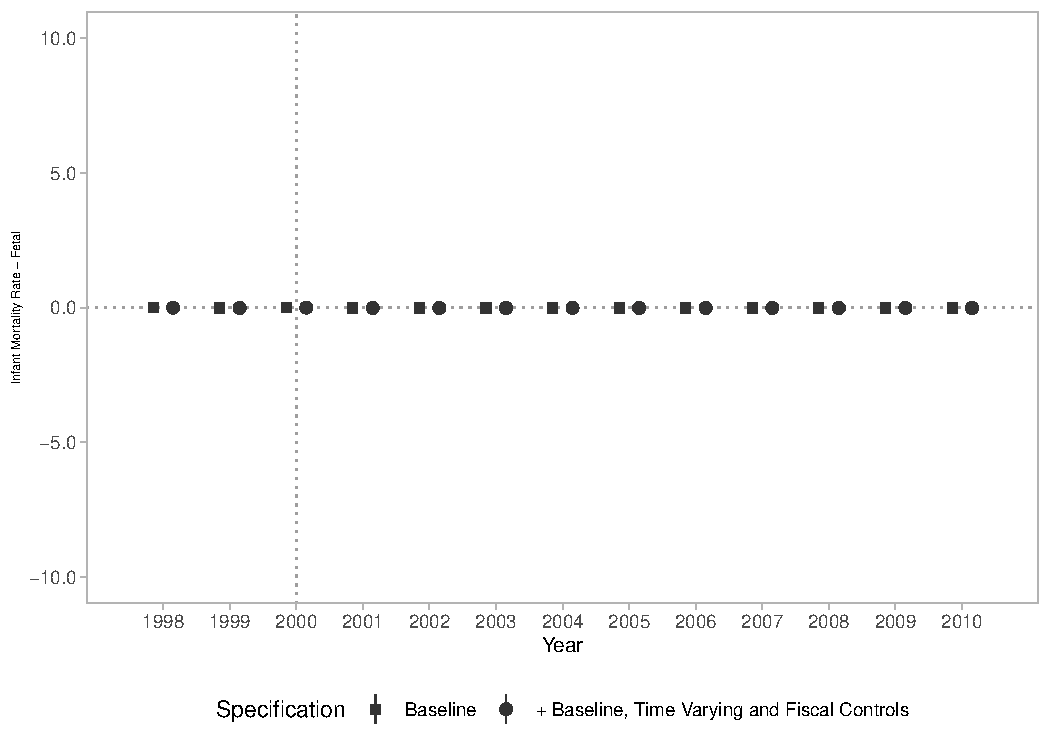
\includegraphics[width=\textwidth]{plots/tx_mi_fet_dist_ec29_baseline_dist_ec29_baseline_17.pdf}
    \end{subfigure}
    \begin{subfigure}{0.48\textwidth}
        \centering
        \caption{\scriptsize Within 24h}\label{fig:17b}
        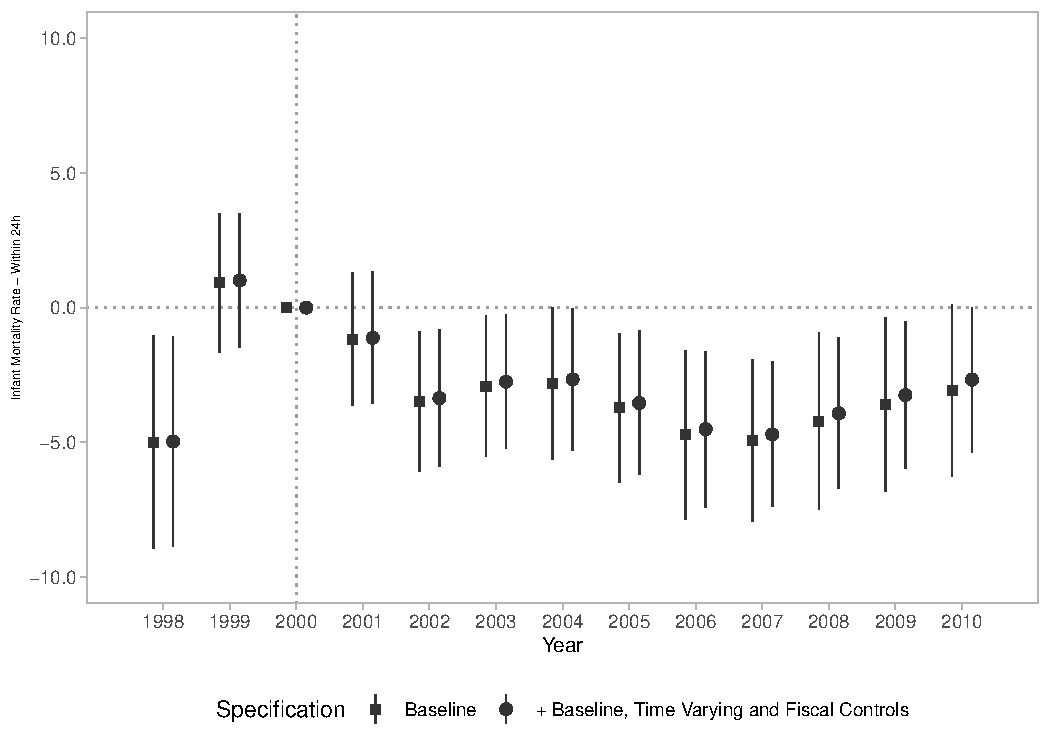
\includegraphics[width=\textwidth]{plots/tx_mi_24h_dist_ec29_baseline_dist_ec29_baseline_17.pdf}
    \end{subfigure}
    \begin{subfigure}{0.48\textwidth}
        \centering
        \caption{\scriptsize 1 to 27 days}\label{fig:17c}
        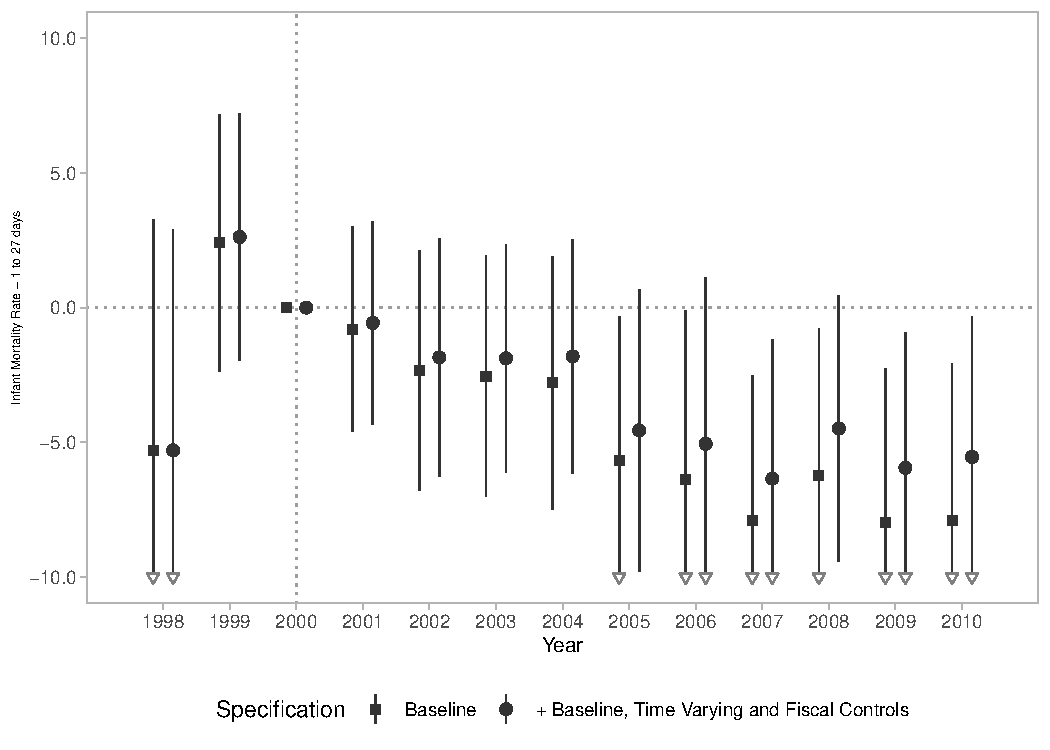
\includegraphics[width=\textwidth]{plots/tx_mi_27d_dist_ec29_baseline_dist_ec29_baseline_17.pdf}
    \end{subfigure}
    \begin{subfigure}{0.48\textwidth}
        \centering
        \caption{\scriptsize 27 days to 1 year}\label{fig:17d}
        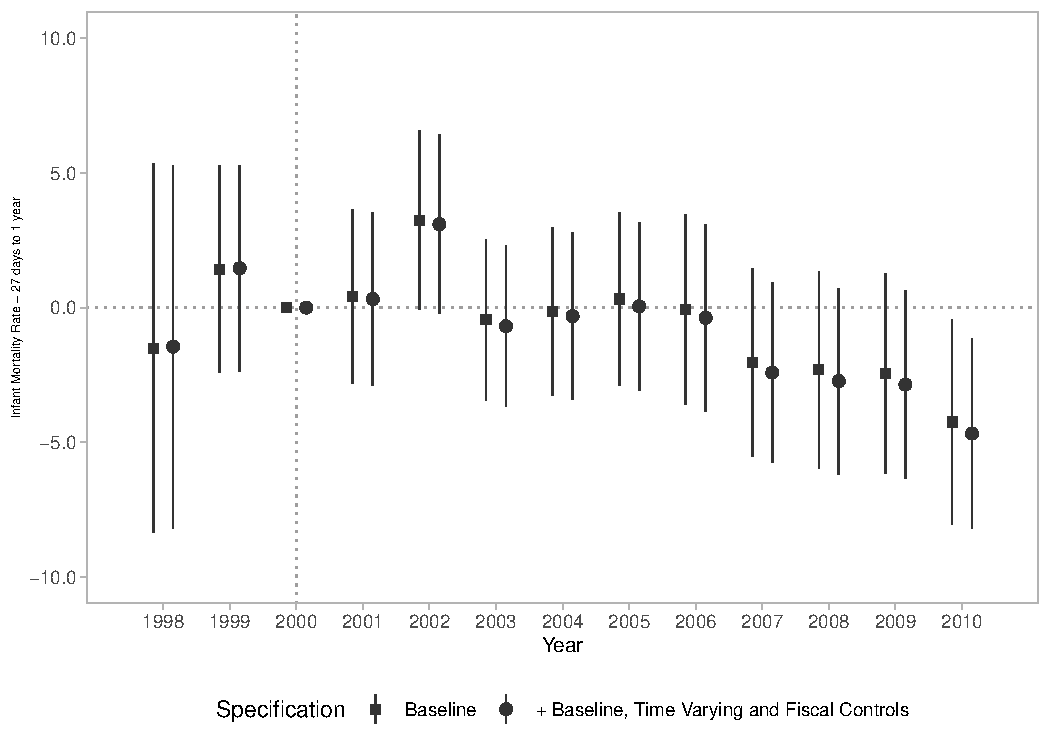
\includegraphics[width=\textwidth]{plots/tx_mi_ano_dist_ec29_baseline_dist_ec29_baseline_17.pdf}
    \end{subfigure}
    
    \end{center}
    
            \scriptsize{Notes: The number of observations is 64701. DiD Estimates from Equation \ref{eq:2}. Independent variable is the distance to the EC/29 target in p.p. Square dots represent the baseline model with municipality and state-year fixed effects. Round dots represent fully saturated specification (Column 4 in regression Tables). Lines represent 95\% confidence intervals. Arrows, when present, indicate confidence intervals out of the plot bounds. Standard errors are clustered in the municipality level.}
    
\end{figure}